\documentclass[main.tex]{subfiles}
\begin{document}
% FIXME FORMELN!
\chapter{Background}\label{chap:Background}
In this chapter, we present relevant literature needed to completely understand the proposed concept of \autoref{chap:Concept}.

\section{SLAM}
SLAM (Simultaneous Localization And Mapping) algorithms aim to solve a usual problem in the field of unmanned robotics;
A robot finds itself in an unknown environment and attempts to build a coherent map while keeping track of its location.
The robot uses use-case-specific sensors to obtain a snapshot of its current surroundings, which it then uses to update and enhance its known map (Mapping).
The robot then attempts to accurately estimate its position based on the updated map. The new information about its position is processed during the next map update.
Over decades of research, varieties of different (combinations of) sensors have been employed to solve this problem more accurately and efficiently.
Internal odometry sensors alone can be unreliable if the robot moves over uneven or slippery surfaces. For that reason, visual SLAM(V-SLAM) methods like \textit{MonoSLAM}\cite{1238654} or
\textit{Dense Visual SLAM}\cite{Kerl_Sturm_Cremers_2013} integrate additional visual input of camera sensors into their algorithm.
% FIXME elaborate
% FIXME Localization
% FIXME top-level Diagram!
% FIXME surveys!

\subsection*{RTAB-MAP}
RealSense-ROS internally uses a SLAM algorithm for map building, namely RTAB-MAP (Real-Time Appearance-Based Mapping)\cite{Labbé_Michaud_2019}.
Unlike purely visual-based SLAM algorithms, RTAB-MAP also takes input from odometry sensors, as well as an optional additional input in form of two- or three-dimensional
lidar scan.
% SECTION 
% FIXME "schon eher grob"
All these inputs are combined during a synchronization step, and the results thereof are passed to RTAB-MAP's \textit{Short-Term-Memory} (STM).
The STM assembles a new node from the new inputs and inserts it into the map graph. Based on the newly inserted node, RTAB-MAP attempts to determine if the current location has already been visited earlier, also known as \textit{loop closure}.
If a loop closure is detected, i.e., RTAB-MAP detects the re-visiting of a known location, the map graph is optimized and thus minimized. In addition, the global map is reassembled in correspondence with the new information.
The resulting map is published in the form of an unorganized point cloud.
% FIXME was ist der unterscheid zwischen OPC und UPC
% !SECTION
RTAB-MAP's general workflow is shown below in Figure~\ref{fig:rtabmap}:
% FIXME integrate figure into previous stanza
% FIXME why is the figure important
\begin{figure}[!h]
    \centering
    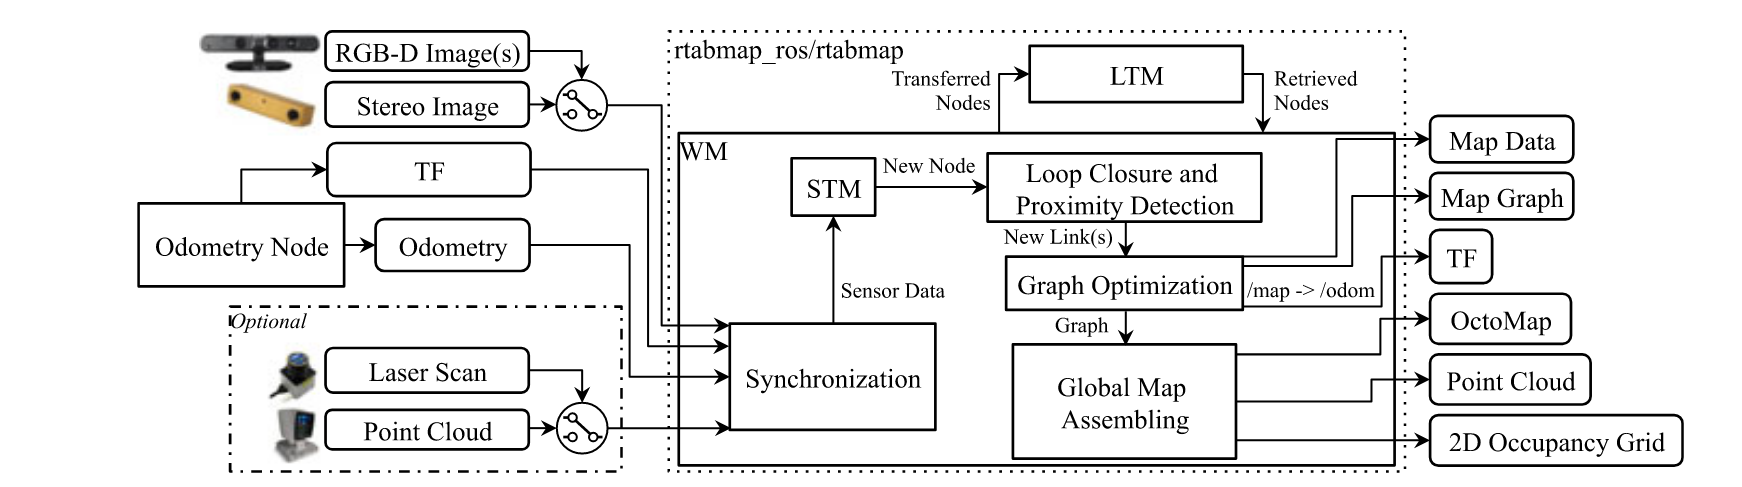
\includegraphics[width=15 cm]{images/rtabmap.png}
    \caption[RTAB-MAP Block Diagram]{Block diagram of RTAB-MAP's main node. Taken from \cite[Figure~1]{Labbé_Michaud_2019}}
    \label{fig:rtabmap}
\end{figure}

\section{Intel Realsense}
In this work, we use the Intel RealSense tracking camera T265 and the RGB-Depth(RGB-D) camera D455.
A tracking camera is generally used to observe the environment and usually has a wider field of view (FOV). The primary motivation for using RGB-D cameras is depth perception.
The primary differences and similarities between the T265 and the D455 are reported in Table~\ref{tab:cameraspecs}.
Beide Kameras sind stereo, die T265 hat 2 fisheye lenses und die D455 hat 2 imagers. Dazu hat die D455 noch einen RGB sensor und einen infrarot sensor. Mit dem IR sensor und den beiden imagern wird ein tiefenbild berechnet.
Durch die fisheye lenses hat die T265 mit 163° ein deutlich breiteres Sichtfeld  als die D455 mit nur 111°. Die maximale FPS anzahl der D455 ergibt sich aus den individuellen FPS werten der imager sensoren und dem RGB sensor, welche beide einen maximalwert von 90 haben.
Dazu sei gesagt, dass bei steigender auflösung die maximale Framerate sinkt und 90FPS nur mit einer maximalen auflösung von 640x480 möglich ist.
Furthermore, both cameras have an integrated Inertial Measurement Unit (IMU) which is used to compute its position in combination with visual input.
% FIXME explain tracking and RGB-D

Intel provides a software development kit, namely RealSense SDK, which allows easy and efficient use of the cameras.
The SDK runs on both Windows and Ubuntu, and a ROS(Robot Operating System \footnote{\href{https://www.ros.org/}{https://www.ros.org/}}) adaptation is also provided in Intel's Github repository \footnote{\href{https://github.com/IntelRealSense/realsense-ros}{https://github.com/IntelRealSense/realsense-ros}}.

\begin{table}[H]
    \centering
    \begin{tabular}{c|ccccccc}
             & Image  & Type     & max. Resolution & D-FOV & Shutter & Price & max. FPS \\ \hline
        D455 & Stereo & RGB-D    & 1280x720        & 111°  & global  & 419\$ & 90       \\ \hline
        T265 & Stereo & Tracking & 848 x 800       & 163°  & global  & 199\$ & 30
    \end{tabular}
    \caption[Intel RealSense T265 & D455 Specification]{Intel RealSense T265 and D455 camera specifications. More information and the complete Datasheets can be found on https://www.intelrealsense.com/.}
    \label{tab:cameraspecs}
\end{table}


\section{Data Formats}
\label{sec:dataformats}
\subsection{Common Input Types}
Usually, the data representation of the recorded environment falls into one of three categories:
\begin{itemize}
    \item \textit{unorganized} or \textit{unstructured point cloud} (UPC)
    \item \textit{organized} or \textit{structured point cloud} (OPC)
    \item image:
          \begin{itemize}
              \item Depth (DI)
              \item RGB (RGBI)
          \end{itemize}
\end{itemize}

The differences between these input types are summarized in Table~\ref{tab:inputs}.
The fundamental difference between UPC and OPC is their format. Each point cloud has a \textit{width} and a \textit{height} parameter.
An unorganized point cloud $c$ is generally equal to an unordered 1D array of 3D coordinates, i.e., $width = |c|$ and $height=1$.
In contrast, the memory layout of an organized point cloud is a 2D matrix, where the width and height depend on the resolution of the used sensor.
Intuitively, the value at index (0,0) would be in the top-left corner, and the value at index (\textit{width,height}) would be in the bottom-right corner.
% FIXME bild selber machen: 2xmatrix mit eintrag, einmal (0,0)=XYZ, einmal (0,0) = d_0,0 

When considering images, a differentiation between RGB images and depth images has to be made.
Depth images are inherently similar to organized point clouds, given their resolution and two-dimensional structure.
The primary difference is that the matrix stores distances to the sensor instead of 3D coordinates.
RGB-images are, like Depth images, stored as a 2D Matrix but instead of distances or coordinates, the matrix stores
values that describe the color of a pixel. Usually, this means that each pixel stores a triple that describes a specific
color by the amount of included red, green, and blue.

Another important aspect is that OPC or images can have 0, empty or \textit{not-a-number} (NaN) entries, while unorganized point clouds
omit such values. Possible reasons for invalid pixels include points too far away from the sensor, or even windows or mirrors.
\begin{table}[H]
    \centering
    \begin{tabular}{c|c|c|c}
        \textbf{Input Type} & \textbf{Value Types} & \textbf{Memory Layout} & \textbf{0 or NaN} \\ \hline
        \textbf{OPC}        & 3D Coordinates       & 2D Matrix              & N                 \\
        \textbf{UPC}        & 3D Coordinates       & 1D Array               & Y                 \\
        \textbf{DI}         & Distances to Sensor  & 2D Matrix              & Y                 \\
        \textbf{RGBI}       & RGB                  & 2D Matrix              & Y
    \end{tabular}
    \caption{Possible inputs for plane detection algorithms columns dedicated to the stored data, the memory layout, and whether
        the input type allows for invalid values.}
    \label{tab:inputs}
\end{table}
It is worth noting that, in the literature, the terms "depth image" and "organized point cloud" are used somewhat
interchangeably.

\subsection{Common Plane Formats}

% FIXME 
\textbf{\textcolor{red}{TODO}}

\section{Plane Detection}
\paragraph*{introduction}
The field of plane detection has been around for decades.
Most methods of detecting planar regions in unorganized point clouds are based on one of three main categories \cite*{\cite{LimbergerOliveira2015HT3D},Araújo_Oliveira_2020}:
\begin{itemize}
    \item Hough Transform (HT)
    \item RANSAC (RC)
    \item Region Growing (RG)
\end{itemize}

\subsection*{Hough Transform}
The original motivation behind the Hough transform was detecting lines in images~\cite{5230799}. All points are sequentially processed via a voting procedure to detect the best fitting line over a set of 2d points.
Multiple lines with different orientations are fit through each given point $p$.
Because a line in slope-intercept form parallel to the y-axis would lead to an infinite slope, the Hesse normal form is chosen as the primary line representation\cite{10.1145/361237.361242}.

In Hesse normal form, an individual line can be parameterized with a pair $(r, \theta)$, with $r$  being the orthogonal distance origin to the plane and $\theta$ being the angle between the x-axis and the line that connects the origin to the closest point on the line.
This pair is also called a \textit{Hough Space} in this context. Votes are cast on the corresponding value of $\theta$, depending on the number of inliers within a specific \textit{Hough Space} $(r_i,\theta_i)$. The map that connects the
votes to each $\theta$ is called an \textit{accumulator}.
Finally, the best fitting line is determined by the number of votes it received.

% FIXME besser schreiben
In the context of plane detection in 3D point clouds, a plane would be uniquely identified by the triple $(\rho, \theta, \phi)$, with $\rho$ being the orthogonal distance from the origin to the plane, $\theta$ being the azimuthal angle, and $\phi$ being the inclination.
Since more parameters are needed to describe a plane in 3D, the accumulator must be adapted.
Therefore, a three-dimensional accumulator is used, whereas the specific shape has been discussed~\cite*{Borrmann_Elseberg_Lingemann_Nüchter_2011}.

\subsection*{RANSAC}
RANSAC (RAndom SAmple Consensus) has been researched for decades. While many use cases revolve around image processing, it is also heavily employed in many plane detection algorithms\cite{Sun_Mordohai_2019, Yang_Forstner, Ashraf_Ahmed_2017}.
RANSAC is an iterative process. Each iteration randomly samples a certain amount of data points and fits a mathematical model through them. The level of outliers determines the quality of the obtained model and preserves the best overall model.

Within the context of plane detection in 3D point clouds, an approach could involve random sampling of 3 points, fitting a plane through them,
and counting the number of points within a certain range of the plane\cite{Yang_Forstner}. The model, in that case, could be a cartesian plane equation.

\subsection*{Region Growing}
Region Growing methods are often used in the field of image or point cloud segmentation \cite{Proença_Gao_2018, Vo_Truong-Hong_Laefer_Bertolotto_2015}.
RG-based segmentation methods aim to grow a set of disjoint regions from an initial selection of seed points. The regions increase in size by inserting neighboring values based on an inclusion criterion.
The quality of the resulting regions depends on the choice of seed points, e.g., a very noisy seed point could decrease overall quality  \cite{Malek_Rahman_Yasiran_Jumaat_Jalil_2012}.
In the context of this work, a criterion for region growth could be the distance or curvature between a region and its adjacent data points.

\section{Plane Detection Algorithms}
The following subsections detail the necessary background knowledge of all the plane detection algorithms mentioned in this paper.
Aside from the functionality of a method, we give relevant higher-level information. \textbf{\textcolor{red}{This includes the separation of an algorithms
        process in pre-processing, plane detection, and post-processing, as well as the expected input format and the proposed output format.}}


\subsection{Robust Statistics approach for Plane Detection}
\label{subsec:bg-rspd}

\textbf{\textcolor{red}{Parameter: $l_O, \varepsilon, MOR, k, MND, MDP$}}

Robust Statistics approach for Plane Detection (RSPD)~\cite{Araújo_Oliveira_2020} is based on region growing. After taking an unorganized point cloud as input, the procedure is divided into three phases;
\textit{Split, Grow and Merge}.

\paragraph*{Split}
The authors propose to use an octree to recursively subdivide the point cloud. The subdivision is repeated until every leaf node contains less than $0.1\%$ of the total amount
of points.
This is followed by a planarity test, during which the octree is traversed bottom-up. If all eight children of a node $n$ are leaf nodes and fail the planarity test, $n$ replaces its children
and becomes a leaf node of its own. This procedure is repeated until the root of the octree is reached.

\paragraph*{Grow}
In preparation for the growth phase, a neighborhood graph (NG) over the entire point cloud is created. Every node of NG represents one point and an edge between two nodes exists only if
a k-nearest-neighbor search detects both points being in the same neighborhood.

The graph construction is subsequently followed by a breadth-first-search, during which a point $x$ is inserted into a planar patch $p$ if it satisfies the following conditions:
\begin{itemize}
    \item $x$ is not included in any patch \textit{and}
    \item $x$ satisfies the inlier conditions for $p$: % FIXME explain them !
          \begin{itemize}
              \item The distance $d$ of $x$ to $p$ is smaller than a threshold $\theta_d$ (see Eq.~\ref{eq:incond1}) \textit{and} % TODO MDP
              \item The angle $\phi$ between the normals vectors of $x$ and $p$ is less than a threshold $\theta_a$ (see Eq.~\ref{eq:incond2}). % TODO MND
          \end{itemize}
\end{itemize}

\begin{equation}
    \label{eq:incond1}
    d = |(x - p.center)\cdot p.normal| < \theta_d
\end{equation}
\begin{equation}
    \label{eq:incond2}
    \phi = acos(|x.normal, p.normal|) < \theta_a
\end{equation}

\paragraph*{Merge}
In the last phase, the previously grown patches are merged. Two planar patches $P_1$ and $P_2$ can be merged, if the following conditions are met:
\begin{itemize}
    \item The octree nodes of $P_1$ and $P_2$ are adjacent,
    \item $P_1.n$ and $P_2.n$ have a divergence within a tolerance range \textit{and}
    \item at least one inlier of $P_1$ satisfies the inlier conditions(see Eq.~\ref{eq:incond1}+\ref{eq:incond2}) from $P_2$ and vice versa.
\end{itemize}

This phase returns all maximally merged planar patches, i.e. the final planes.

\subsection{Oriented Point Sampling}
Oriented Point Sampling (OPS)~\cite{Sun_Mordohai_2019} accepts an unorganized point cloud as input.

\textbf{\textcolor{red}{more detail}}
\textbf{\textcolor{red}{parameters: $\alpha_s, KNN, \theta_h, \theta_N, p$}}

First, a sample of points is uniformly selected. The normal vectors of these points are estimated using SVD and the k nearest neighbors, which had been obtained using a k-d tree.
An inverse distance weight function is employed to prioritize neighboring points that are closer to the sample of which the normal vector is currently being estimated.


After normal estimation, one-point-RANSAC is used to find the largest plane. Usual RANSAC implementations sample three points to fit a plane. However, OPS fits a plane with only one sample point and its normal vector.
Once a plane with the most inliers is obtained, its normal vector is re-estimated using SVD on all inliers, and all inliers are removed from the point cloud.
This process is repeated until the number of remaining points falls below a predefined threshold $\theta_N$.
% FIXME
\textbf{\textcolor{red}{post-processing}}
\begin{itemize}
    \item merge smaller planes if they pass a coplanarity test
    \item re-estimate normals after merge
\end{itemize}

\subsection{3D Kernel-based Hough Transform}\label{sub:3dkht}
With the 3D Kernel-based Hough Transform (3D-KHT),
\citeauthor{LimbergerOliveira2015HT3D}\cite{LimbergerOliveira2015HT3D} propose a hough transform-based plane detection method,
which accepts unorganized point clouds as input \cite{LimbergerOliveira2015HT3D}.

\textbf{\textcolor{red}{parameters: $\phi_{num}$  $\rho_{num}$  $s_{level}$  $s_{ps}$  $d_{max}$     $s_\alpha$  $s_\beta$}}

The point cloud is spatially subdivided. The authors propose the usage of octrees over k-d trees because the k-d tree lacks efficiency in creation and manipulation.
Furthermore, the octree succeeds in capturing the shapes inside the point cloud, while the k-d tree does not.

Each leaf inside the octree continues subdividing until the points inside a leaf node are considered approximately coplanar, or the number of points is less than a predefined threshold.
The authors recommend this threshold to value 30 for large point clouds.
After the approximately coplanar nodes are refined by removing outliers, a plane is fit through the remaining points.


This plane $\pi$ can, in polar coordinates, be uniquely described by a triple $(\rho, \theta, \phi)$.
Inspired by \citeauthor{Borrmann_Elseberg_Lingemann_Nüchter_2011}\cite{Borrmann_Elseberg_Lingemann_Nüchter_2011}, an accumulator ball (Fig.~\ref{fig:accball}) is used for the voting procedure because the cells in polar regions are smaller (and therefore
contain fewer normal vectors) in three-dimensional accumulator arrays, as portrayed in Figure~\ref{fig:accarr}.


\begin{figure}[H]
    \centering
    \hspace{\fill}
    \begin{subfigure}{0.25\textwidth}
        \centering
        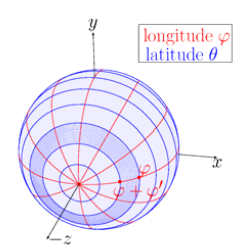
\includegraphics[width=\textwidth]{images/accumulatorarray.png}
        \caption[3D-KHT Accumulator Array]{}
        \label{fig:accarr}
    \end{subfigure}
    \hspace{\fill}
    \begin{subfigure}{0.25\textwidth}
        \centering
        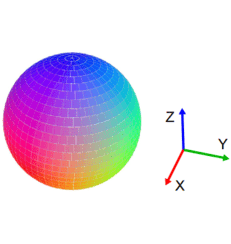
\includegraphics[width=\textwidth]{images/accumulatorball.png}
        \caption[3D-KHT Accumulator Ball]{}
        \label{fig:accball}
    \end{subfigure}
    \hspace{\fill}
    \caption[Hough Transform Accumulators]{Accumulator array (a), taken from \cite*[Figure~3]{Borrmann_Elseberg_Lingemann_Nüchter_2011}. Accumulator
        ball(b) used in 3D-KHT, taken from \cite*[Figure~5]{\cite{LimbergerOliveira2015HT3D}}.}
\end{figure}

During the voting procedure, votes are not cast for each data point but rather on previously calculated approximately coplanar clusters.
When casting a vote on a given cluster $c_i$ with its plane (represented by $(\rho, \theta, \phi)$), the corresponding entry in the accumulator ball is updated.
With this update, its neighboring clusters also receive a vote determined by the uncertainty value of $c_i$. Due to the non-discrete
values of uncertainty, the votes are floating-point values as well.

All Peaks within the accumulator ball are detected in the last step. Because the votes tend to be sparsely distributed \cite[Section~3.4]{\cite{LimbergerOliveira2015HT3D}},
an auxiliary array $A$ is used to memorize the entries inside the accumulator that are set. When an accumulator index is assigned a value for the first time, it is also added to $A$.
Therefore, it is only necessary to iterate the auxiliary array to find peaks inside the accumulator.
Furthermore, an intermediary smoothing step is performed by merging adjacent peaks inside the accumulator and storing them in $A$.
Then, $A$ is sorted in descending order.
If a cell $c$ in the accumulator has not yet been visited during iteration, $c$ is considered a peak. In addition, $c$ and its 26 neighboring cells are tagged as \textit{visited}.
That way, the most dominant plane, i.e., the one with the most votes, is detected first.
Finally, the detected planes are sorted by the number of different clusters that voted for them.

\subsection{Octree-based Region Growing}
\label{subsec:bg-obrg}
Octree-Based Region Growing (OBRG) \cite{Vo_Truong-Hong_Laefer_Bertolotto_2015} is also a method that employs region growing.

\textbf{\textcolor{red}{parameters: $l_{max}$ $\theta_{res}$  $\theta_{d}$  $\theta_{ang}$  $\theta_M$  $\theta_p$}}

First, an unorganized point cloud is recursively subdivided using an octree.
An octree node $n$ repeatedly subdivides itself into eight children until the level of $n$ supersedes a predefined maximum subdivision value or if the
amount of contained points in $n$ is less than a predefined minimum of included points.
Saliency features are calculated for every leaf node in preparation for the region growing step. A normal vector is obtained by performing a principle
component analysis (PCA) on the points inside each leaf node. The best-fitting plane of each leaf is defined by the mean normal vector and its center point.
A residual value is obtained by taking the RMS of the distance of all included points to the plane.

For the region growing phase, all leaf nodes are selected as individual seed points. Starting from the seed with the lowest residual value, which relates to a low amount of noise,
a neighboring leaf node $n$ is inserted into the region if $n$ does not belong to any region and the angular divergence between both normal vectors is smaller than
a predefined threshold.
% FIXME explain inlier criteria, mention thresholds
Lastly, a refinement step is employed.
Fast refinement (FR) is performed on regions that succeed in a planarity test, i.e., 70\%-90\% of included points fit the best plane~\cite[Section~3.4]{Vo_Truong-Hong_Laefer_Bertolotto_2015}. FR is leaf-based, and all previously unallocated neighboring nodes that satisfy an inlier criterion are added to the region.
General refinement (GR) is performed on regions that are considered non-planar. In contrast to the fast refinement, GR is point based. Therefore,
points from neighboring and previously unallocated leaf nodes are considered and inserted into the region if they, too, satisfy the inlier criterion.
The refinement process returns a complete set of planar regions.

\subsection{Probabilistic Agglomerative Hierarchical Clustering}
\label{subsec:bg-peac}
Probabilistic Agglomerative Hierarchical Clustering (PEAC)~\cite{Feng_Taguchi_Kamat_2014} is a plane detection algorithm that takes an organized
point cloud as input.
The agglomerative hierarchical clustering is based on an algorithm called
\textit{line regression}\cite[Section~III.B]{Nguyen_Martinelli_Tomatis_Siegwart_2005}. The primary difference is
that, instead of a double linked list, PEAC operates on a graph $G$.

First, the input organized point cloud is divided into non-overlapping nodes through the initialization of $G$.
Each node in $G$ has a pre-determined height $H$ and width $W$, whereas $H$ and $W$ correspond to index ranges in the
point cloud, i.e., each node contains a set of points.
Then, $G$ is refined by removing the following types of nodes and corresponding edges~\cite[Section~III.A]{Feng_Taguchi_Kamat_2014}:
\textbf{\textcolor{red}{zitieren um depth discontinuities sagen zu dürfen?}}
\begin{enumerate}
    \item Nodes that contain NaN or 0 values, e.g., missing data,
    \item nodes that contain at least one point that is depth-discontinuous with its four neighbors, e.g., neighbors
          in the pixel space but not in coordinate space,
    \item nodes with a high MSE, e.g., non-planar regions, \textit{and}
    \item nodes that share an edge with two different planes, e.g., the corners of walls.
\end{enumerate}
During this step, all points inside a node share a common plane normal.

The \textit{agglomerative hierarchical clustering} step starts with the construction of a min-MSE-heap data
structure that contains the nodes of $G$, sorted in ascending order by the value of their MSE.
The following steps are then repeated exhaustively.
First, the node $v$ that has the current minimum MSE is merged with one of its neighbors $u$ that minimizes the merged MSE.
If the merged MSE is larger than a threshold $\theta_{MSE}$, then a plane is found and the merged node is removed from G.
if $MSE_{merge}$ is larger than a threshold $\theta_{MSE}$, then a plane segment is found and extracted from $G$.
Otherwise, the merged node is added back to $G$, joining the edges of $v$ and $u$.

Lastly, a refinement step is employed. Due to the clustering of nodes that contain a set of points, certain types of
artifacts can occur:
\begin{itemize}
    \item Sawtooth,
    \item unused data points, \textit{and}
    \item over-segmentation.
\end{itemize}
First, if not all neighbors of a node $v$ belong to the plane of $v$, all points of $v$ are added to a queue $Q_{RG}$.
Then, region growing is performed on the points inside $Q_{RG}$, where the 4-connected neighbors are observed.
A neighboring point $n$ is inserted into the segment $k$ of a point $v$ if $n$ does not belong to $k$, and
the distance to $k$ is smaller than the distance to its current segment. Additionally, $n$ is inserted into $Q_{RG}$,
which also happens if $n \in k$.
The region growing is followed by another \textit{agglomerative hierarchical clustering} step.


\subsection{Fast Cylinder and Plane Extraction}
Fast Cylinder and Plane Extraction (CAPE)~\cite{Proença_Gao_2018} is a region growing-based algorithm that detects
planes and cylinders in organized point clouds.
The authors propose this algorithm as an extension of their Probabilistic Visual Odometry Framework~\cite{Proenca_Gao_2018}.

In preparation for the region growing step, the cloud is subdivided into patches of pre-defined size, similar to
the graph initialization of PEAC (see Section~\ref{subsec:bg-peac}).
A patch size of 20x20 was used in their evaluation~\cite[Section~V.A]{Proença_Gao_2018}.
Then, the planarity of the patches is tested, and a patch is considered non-planar, if:
\begin{itemize}
    \item The amount of NaN or 0 points exceeds a threshold, \textit{or}
    \item the patch has depth discontinuities,
\end{itemize}
whereas the depth discontinuities are only checked for pixels along two vertical and horizontal lines that pass through
the patch center. \textbf{\textcolor{red}{satz ist schon sehr ähnlich zum original}}
A plane is then fit through the patch inliers by performing principle component analysis (PCA). The plane's MSE
corresponds to the lowest eigenvalue, and the plane's normal vector is its eigenvector.
A patch is considered planar, if:
\begin{equation}
    MSE_{patch} < (\sigma_{\bar{z}} + \epsilon)^2,
\end{equation}
where $\sigma_{\bar{z}}$ is the estimated standard uncertainty of the patches' mean depth value. $\epsilon$ is a
tolerance coefficient. \textbf{\textcolor{red}{satz ist schon sehr ähnlich zum original}}

The normal vectors are converted from cartesian to spherical coordinates, thus being described by a polar angle, and
an azimuth angle. These spherical normal vectors are then assorted into bins, thus building a histogram $H$.

This histogram is now used for the region growing step.
First, a set of patches $C$ of the most frequent bin in $H$ are obtained. Stop, if the most frequent bin
yields fewer patches than a threshold $k_1$. The patch with the smallest MSE out of $C$ is chosen as a seed $s$.
In general, a 4-connected neighborhood is used in this approach, and a neighboring patch $n$ is inserted into a region, if:
\begin{enumerate}
    \item $n$ is not assigned to any region,
    \item the dot product of both patches normal vectors is less than a threshold $T_N$, \textit{and}
    \item the orthogonal distance of $n$'s center to the region is less than $T_d(s) = l\sqrt{(1-T_N^2)}$,
\end{enumerate}
where $l$ is the distance between the corner points of $s$.
If a complete segment $S$ is found, all included patches are removed from the list of remaining patches, and
the bins of the histogram are updated accordingly. Lastly, if $S$ exceeds the minimum plane size $k_2$, it is added
to the set of detected planes.

The planarity of all segments is now assessed. This is done by calculating the covariance of all included points and,
subsequently, comparing the ratio of the second largest eigenvalue to the smallest eigenvalue thereof. If this ratio
exceeds a pre-determined parameter $plane_min_score$, the segment is considered a plane.
Otherwise, additional steps are needed.
First, the surface of a segment is checked for invariance, which is a property of open cylinders.
For this task, PCA is performed on the stacked matrix of normal vectors of the segment.
Then, the ratio of the first eigenvalue to the last eigenvalue of this covariance matrix, namely the condition number,
is calculated. If the condition number exceeds a threshold $\theta_{cond}$, the segment is comprised of a set of
cylinders or planes~\cite[Section~III.D]{Proença_Gao_2018}.

Using the eigenvector with the smallest eigenvalue, the center points and normal vectors of all patches
in the segment are then projected onto a plane. Then, multiple models are fit by performing sequential RANSAC.
Planes are then fit through each model obtained by RANSAC. If the MSE of the plane is lower than the MSE of
the corresponding cylinder model, the model is considered a plane, and a cylinder otherwise.

Lastly, the segments are undergone a refinement step.
First, segments are eroded by removing boundary patches through the use of a 3x3 kernel. Next, the eroded segments are expanded by using
a 3x3 8-neighbor kernel. The authors propose, that all patches valid for refinement are given by the difference between
the expanded segment and the eroded segment. Lastly, each pixel $p$ within the patches is added to
the segment $S$ if:
\begin{equation}
    dist(p,S) \leq MSE_S \cdot k,
\end{equation}
where $k$ is a constant. The authors use $k=9$ in their work.

\subsection{Plane Extraction using Spherical Convex Hulls}
As the name suggests, Plane Extraction using Spherical Convex Hulls (SCH-RG) employs spherical convex hulls to
detect planes in organized point clouds.
The primary concept behind this method is that the planes are not parameterized, but rather represented as
a set of geometric constraints in the spherical coordinate system.

First, a set of pre-processing steps is employed.
First, a bilateral filter is used for the reduction of noise. Subsequently, a normal map of the entire image
is generated.
To prepare for the region growing step, appropriate seeds are selected. This is effectively done by subdividing the
image into a grid, discarding non-planar cells, and choosing the cell centroids as seeds.
The planarity of a cell is determined by its mean-square-error (MSE), which is calculated through all included
points and the best fitting plane. This MSE is then compared against a MSE threshold.

Having obtained a set of seed points, the region growing step is employed.
Each time a new seed is retrieved, all normals of the corresponding cell are gathered and transformed
into the spherical domain. A queue is used for the retrieval of seeds and neighboring points.
Starting from a seed $s$, neighboring points and their normals are sequentially retrieved.
If a neighbor $n$ is already assigned to some region or the depth difference is larger than a threshold $T$, it is
discarded. If $n$ is located inside of the spherical convex hull of the region of $s$,
it is added to the region, and its neighbors are inserted into the queue. If $n$ is not inside a
convex hull, it is necessary to check whether $n$ is outside of the so-called \textit{cluster-permissible region} (CPR):
\begin{equation}
    CPR(p) = \{q \in \mathbb{S} | \angle(p,q)\leq 2\theta\},
\end{equation}
where $\theta$ is an angular threshold. Note that the CPR of multiple points, e.g., a region, is determined by
the intersection of all individual points.
If $n$ is outside the CPR of the current region, it is discarded. Otherwise, the convex hull is updated with $n$,
$n$ is added into the set of points included in the region, and its neighbors are inserted into the queue.
It is worth noting, that seed points that are associated with already detected planes are discarded upon retrieval.

Lastly, dilation is performed to eliminate holes in planes. This is not further detailed in~\cite[Section~III.B]{Mols_Li_Hanebeck_2020}.


\subsection{Depth Kernel-based Hough Transform}
Depth Kernel-based Hough Transform (D-KHT) \cite{Vera_Lucio_Fernandes_Velho_2018} is a Hough transform-based plane detection
algorithm that accepts depth images as input.

\textbf{\textcolor{red}{pre-processing}}
clustering:
\begin{itemize}
    \item quadtree subdivision
          \begin{itemize}
              \item whole image is root
              \item each node with more than threshold $s_{ms}$ samples: coplanarity test with PCA
              \item all nodes with less than $s_{ms}$ inliers are ignored in the voting process
              \item
          \end{itemize}
    \item Summed area tables (SAT) computation for PCA efficiency
          \begin{itemize}
              \item the covariance and mean values can be calculated in constant time that way
              \item pre-compute (9) SATs for each node
          \end{itemize}
\end{itemize}

\textbf{\textcolor{red}{plane detection}}
given set of approx coplanar point clusters in leaf node
\begin{itemize}
    \item the best fitting plane is described by its mean point and a unit normal vector (which is the
          associated eigenvector to the least eigenvalue of the cov matrix)
    \item the gaussian kernel that weights votes from the cluster in the parameter space of the plane normal
    \item calc cov matrix of the gaussian kernel can be computed with first order error propagation \textbf{\textcolor{red}{mathe}}
    \item cluster votes in spherical accumulator map $A$
          \begin{itemize}
              \item $\theta \in [-\pi , +\pi], \phi \in [0, \pi], \rho \in [0, \rho_{high}]$
              \item $\rho_{high}$ is the farthest point from camera to a sample
              \item the amount of samples within rho and are defined by params $N_\rho, N_\phi$
          \end{itemize}
    \item voting:
          \begin{itemize}
              \item for given kernel that is associated with a cluster:
              \item increment bins of A that fall within two standart deviations of the mean \textbf{\textcolor{red}{formel}}
              \item starting at specific bin, neighbors are flood filled with \textbf{\textcolor{red}{mathe}} als termination condition
          \end{itemize}
    \item after voting:
          \begin{itemize}
              \item compute convolution of accumulator with six-connected filter (smoothing of map)
              \item hill climbing to detect peaks: plane is detected if the bin of a mean plane is a local maxima
          \end{itemize}
\end{itemize}

\textbf{\textcolor{red}{post processing}}
given set of parameters corresponding to detected planes
\begin{itemize}
    \item sort planes by relevance
    \item relevance is defined by the summation of the weights associated with the clusters that contributed to the peak
\end{itemize}
The normal vector and the distance $\rho$ define the normal equation of the plane supporting a subset of
3d point entries.


\subsection{Depth Dependent Flood Fill}
\textbf{\textcolor{red}{another case of "nicht perfekt verstanden, daher zu lang". reicht aber als erste iteration}}
Depth Dependent Flood Fill (DDFF)~\cite{Roychoudhury_Missura_Bennewitz_2021_new} is a region growing-based algorithm that detects planes in organized point clouds.
The algorithm builds upon and improves their previous method~\cite{Roychoudhury_Missura_Bennewitz_2021_old}.

The algorithm starts by selecting appropriate seeds. First, the organized point cloud gets subdivided into cubes of a
pre-determined size $\sigma_{seed}$. Within these cubes, the points are checked for depth discontinuities, as well as
curvature discontinuities. They are evaluated against $\sigma_{seed}$ and a normal orientation difference
threshold $\theta_{ang}$, respectively. If neither of the thresholds are exceeded, the center of the cube is marked as
a seed for region growing.

The region growing is performed on point-level. Starting from a given seed $s$, a region is expanded by checking
neighbors within a horizontal span.
Given a horizontal span of length n, its middle pixel $p$, the minimum plane size $\sigma$ is calculated as follows:

\begin{equation}
    \sigma = \rho(p) = \kappa_\rho \cdot \delta(p)^2 + \gamma_\rho,
\end{equation}
where $\delta(p)$ is the depth value of $p$, and $\kappa_\rho, \gamma_\rho$ are tuneable parameters.
If the span is growing towards the right, the pixel $n$ that is $\sigma$ pixel away from the right border is checked
for membership. Additionally, $n$'s upper and lower neighbors are also checked for membership. If $n$ and at least one
of $n$'s vertical neighbors pass the following membership test, $n$ and all pixels in between are added to the span of $s$.

\begin{enumerate}
    \item The perpendicular distance of $n$ to the plane defined by $s$ and its normal is smaller than
          a threshold $\tau_{flood}$,
    \item the euclidian distance between $p$ and a neighboring pixel is smaller than a threshold
          $\tau_{point}$, \textit{and}
    \item $n$ is neither NaN, nor 0.
\end{enumerate}

This region growing process yields a set of oversegmented planes. In a refinement step, the set of planes is reduced
by performing merging of planes.
First, a neighborhood graph of the rough segments is constructed. Any segments that share a border, i.e., the bordering
pixels have a small euclidian distance, are connected through a bidirectional edge.
The graph is traversed in a breadth-first manner, merging two connected nodes, $a,b$, if they satisfy the following condition:

\begin{enumerate}
    \item the seed normals of a and b diverge less than a threshold $\tau_{angle}$, \textit{and}
    \item the perpendicular distance between the segments is less than threshold $\tau_{merge}$.
\end{enumerate}
If $a$ fails the membership test with its neighbor $b$, the membership test is repeated between $b$ and all planes $a$
has merged with. If this fails, the unidirectional edge $(ab)$ is removed from the graph. Note, that the edge $(ba)$ will
be validated later, as b is subject to change through merges with other neighbors.

After a successful merge, a new centroid and normal are obtained by adding both plane normals and centroids together,
while the respective amount of inliers acts as a weight.

The BFS iteration is repeated, until no merge occurs during an iteration. The authors state that, typically, no more than five
iterations are needed~\cite[Section~III.E]{Roychoudhury_Missura_Bennewitz_2021_new}.

The flooding under the constraint of minimum plane size leaves gaps. Therefore, as a refinement step, a two-pass
algorithm is used to fill these gaps. The first pass scans top-to-bottom, and the second bottom-to-top.
In both passes, horizontal strips of non-assigned pixels are detected. If the vertical neighbors have the same plane label,
we mark all unmarked pixels with the same label.

\subsection{PlaneNet}
PlaneNet~\cite{Liu_Yang_Ceylan_Yumer_Furukawa_2018} ist a deep learning-based approach to piece-wise planar reconstruction of a scene from a single RBB-Image.

\textbf{\textcolor{red}{hier würde sich wahrscheinlich die grafik anbieten}}
\begin{itemize}
    \item built upon Dilated Residual Networks (DNR)
    \item followed by three predicion tasks
          \begin{enumerate}
              \item plane parameters
                    \begin{itemize}
                        \item global average pooling, reduce feature map size to 1x1
                        \item fully connected layer to produce Kx3 plane parameters. (K=10 in experiments)
                        \item loss function: order agnostic, based on chamfer distance metric for regressed plane parameters
                    \end{itemize}
              \item segmentation mask
                    \begin{itemize}
                        \item start: pyramid pooling module
                        \item then: convolution layer. produces K+1 channel likelihood maps for planar and non-planar surfaces
                        \item finally: Dense conditional random field (DCRF), based on fast inference. meanfield iterations: 5/10 (training/testing)
                        \item loss function: softmax cross entropy to supervise segmentation training (pixel level)
                    \end{itemize}
              \item non-planar depthmap
                    \begin{itemize}
                        \item start: pyramid pooling module
                        \item followed by convolution layer, produces a 1-channel depthmap
                        \item loss function: sum of squared depth differences between GT and predicted plane or non-planar
                              depthmap (weighted by probabilities)
                    \end{itemize}
          \end{enumerate}
\end{itemize}

\subsection{PlaneRecNet}
PlaneRecNet~\cite{Xie_Shu_Rambach_Pagani_Stricker_2022} is a deep learning-based approach for piece-wise plane detection and reconstruction that takes RGB images
as input.
\begin{figure}[H]
    \centering
    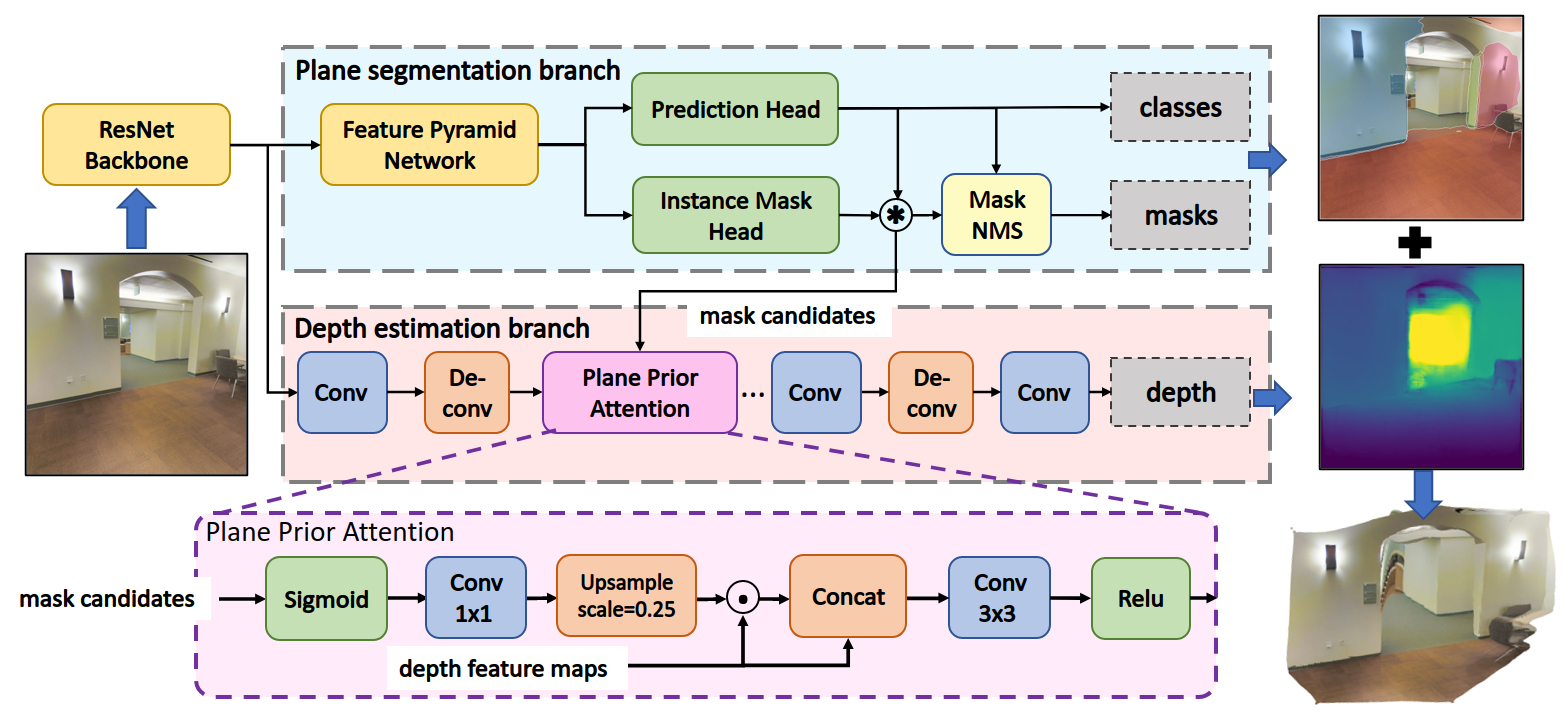
\includegraphics[width=\textwidth]{images/planerecnet.png}
    \caption[PlaneRecNet Architecture]{The PlaneRecNet Architecture. Taken from the respective paper~\cite{Xie_Shu_Rambach_Pagani_Stricker_2022}.
        \textbf{\textcolor{red}{die grafik gibts evtl nochmal in scharf im repo}}}

    \label{fig:planerecnet}
\end{figure}

approach:
focus on high quality global depth estimation so that plane params can be computed by PCA or RANSAC with the plane
segmentation and depth prediction.

\begin{itemize}
    \item ResNet backbone output as input for the following
    \item two seperate branches
          \begin{itemize}
              \item plane segmentation branch
                    \begin{itemize}
                        \item in general: leight weight configuration of SOLOV2 \cite{wang2020solov2} adapted for planar segmentation
                        \item more specific: Feature pyramid network, followed by a prediction head and an instance mask head
                        \item returns classes (obt. from pred. head)
                        \item and masks obt. from non maximum suppresion of pred head and inst. mask head
                    \end{itemize}
              \item depth estimation branch
                    \begin{itemize}
                        \item repeated convolution and de-convolution
                        \item after the first iteration: plane prior attention module with mask candidates as input which are obtained
                              from dynamic convolution between the prediction head and instance mask head from the plane segmentation branch
                        \item finally: returns depth
                    \end{itemize}
              \item plane prior attention module:
                    \begin{enumerate}
                        \item sigmoid function
                        \item 1x1 convolution
                        \item upscale(=0.25) with interpolation
                        \item multiplication and concatenation of mask candidates with depth feature maps
                        \item concatenation of monocular depth estimation and depth feature maps
                        \item 3x3 convolution
                        \item relu activation
                    \end{enumerate}
          \end{itemize}
    \item i guess classes+masks are combined into planes
    \item which is combined with the depth for a reconstructed scene
\end{itemize}


\subsection{PlaneRCNN}
RCNN~\cite{Liu_Kim_Gu_Furukawa_Kautz_2019} is a deep neural architecture that detects planar
regions and reconstructs a piecewise planar depth map from RGB-Images.

\begin{figure}[H]
    \centering
    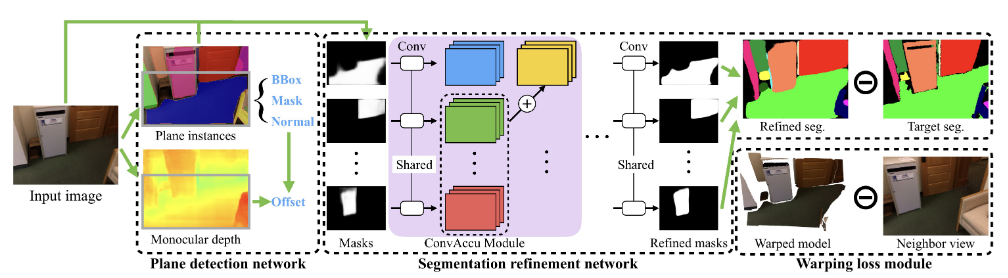
\includegraphics[width=\textwidth]{images/planercnn.png}
    \caption[PlaneRCNN Architecture]{The PlaneRCNN Architecture. Taken from the respective paper~\cite{Liu_Kim_Gu_Furukawa_Kautz_2019}.
        \textbf{\textcolor{red}{die grafik gibts evtl nochmal in scharf im repo}}}
\end{figure}

3 main components:
\begin{enumerate}
    \item plane detection network
          \begin{itemize}
              \item predicts 3d plane parameters and segmentation mask
              \item built upon Mask-R-CNN. here: "planar" as object instance
              \item maskrcnn detects instances and estimates segmentation masks
              \item then, estimate plane normal and offset $d$:
                    \begin{enumerate}
                        \item predict normal per planar instance
                        \item estimate depth map
                        \item algebraically calculate plane offset \textbf{\textcolor{red}{formel?}}
                    \end{enumerate}
          \end{itemize}
    \item segmentation refinement network
          \begin{itemize}
              \item takes the planar regions from 1. and optimizes the masks
              \item uses convAccu: combines convolution layer and an accumulation scheme
              \item aggregates information from all masks
              \item at the end, refined plane masks are concatenated and compared against target
                    masks with a cross entropy loss
          \end{itemize}
    \item warping loss module (only during training)
          \begin{itemize}
              \item uses a second angle on the same scene to ensure consistency
              \item nearby view is 20 frames ahead during training
              \item calculate nearby view by warping every pixel in the nearby view to the current one
                    given the camera intrinsics
              \item loss function is a simple absolute error between the current view and the
                    warped nearby view.
          \end{itemize}
\end{enumerate}

\section{Datasets}
This section outlines a set of datasets popular in the evaluation of algorithms
in the field of plane detection. Table~\ref{tab:datasets} summarizes the key characteristics of each
dataset. The individual datasets are outlined in the following subsections.
% FIXME Datensätze erklären
% FIXME Tabelle erläutern!
% \begin{table}[H]
%     \centering
%     \begin{tabular}{c|c|c|c|c}
%         \textbf{Dataset}                                                                                                                                                                      & \textbf{Input Format} & \textbf{Real} & \textbf{Indoor} & \textbf{GT} \\ \hline
%         \textbf{SegComp}     \cite{article}                                                                                                                                                   & DI                    & N             & /               & planes      \\
%         \textbf{2D-3D-S}      \cite{2017arXiv170201105A}                                                                                                                                      & UPC                   & Y             & Y               & objects     \\
%         \textbf{NYU V2}      \cite{10.1007/978-3-642-33715-4_54}                                                                                                                              & DI                    & Y             & Y               & classes     \\
%         \textbf{Kinect}      \cite{Oehler_Stueckler_Welle_Schulz_Behnke_2011}                                                                                                                 & OPC                   & Y             & Y               & planes      \\
%         \textbf{ICL-NUIM}    \cite{handa:etal:ICRA2014}                                                                                                                                       & DI                    & Y             & Y               & trajectory  \\
%         \textbf{SYNBEP}      \cite{schaefer19icra}                                                                                                                                            & OPC                   & N             & /               & planes      \\
%         \textbf{ARCO}        \cite{Hidalgo-Paniagua_Vega-Rodríguez_Pavón_Ferruz_2015}                                                                                                         & OPC                   & Y             & Y               & /           \\
%         \textbf{SUN}         \cite{7298655}                                                                                                                                                   & DI                    & Y             & Y               & objects     \\
%         \textbf{Leica\tablefootnote{\href{https://shop.leica-geosystems.com/de/leica-blk/blk360/dataset-downloads}{https://shop.leica-geosystems.com/de/leica-blk/blk360/dataset-downloads}}} & UPC                   & Y             & N               & planes      \\
%         \textbf{TUM}         \cite{sturm12iros}                                                                                                                                               & DI                    & Y             & Y               & trajectory
%     \end{tabular}
%     \caption[Popular Datasets]{Popular Datasets. The \textit{GT}(Ground Truth) column specifies what the ground truth of each dataset represents.
%         Note, that the synthetic datasets (e.g., SegComp and SYNBEP) represent neither indoor nor outdoor scenes, hence the "/" in
%         the respective table entries.
%     }
%     \label{tab:datasets}
% \end{table}

\subsection{SegComp}
\subsection{2D-3D-S}
\label{subsec:bg-stanford}
\textit{2D-3D-S} was recorded in three different buildings and divided into six distinct areas, including 272 different scenes. A detailed statistic of the included scene types can be found in Table~\ref{tab:stanfordStats}.
An individual scene has a complete unstructured point cloud and a list of annotated files representing semantically different objects that can be found therein.
The dataset includes a wide range of point cloud sizes, with a minimum of $8\cdot 10^4$ and a maximum of $7\cdot 10^6$
Furthermore, the average amount of points per scene is ${\sim}10^6$ with an average file size of ${\sim}34mb$.

\textcolor{red}{diese 2 sätze sind dann jetzt wahrscheinlich misplaced}
Furthermore, one could argue that an uneven distribution of scene types introduces a particular bias. While it is true that the distribution is quite uneven, the dataset nevertheless reflects a realistic distribution of scene types since
it is not realistic if a building contains only lecture halls. Inversely, it is appropriate to assume that an office complex contains a substantial amount of hallways needed to connect all offices.

\subsection{NYU V2}
\subsection{Kinect}
\subsection{ICL-NUIM}
\subsection{SYNBEP}
\subsection{ARCO}
\subsection{SUN}
\subsection{Leica}
\subsection{TUM}


\section{Evaluation Metrics}
\label{sec:metrics}
Wenn man sachen segmentiert oder muster erkennen möchte usw. benutzt man oft zur evaluierung metriken, die die qualität der benutzten methode beschreiben.
Usual metrics are \textit{precision, recall} and the \textit{f1-score}.
In general, \textit{precision} describes how many of the results are relevant, i.e., the percentage of correctly calculated values(see Eq.~\ref{eq:prec}). \textit{Recall} describes the ratio of relevant results to all relevant data, i.e.
the likelihood of a result being relevant(see Eq.~\ref{eq:rec}). Lastly, the \textit{f1-score} is the harmonic mean of the former two metrics (see Eq.~\ref{eq:f1}).

\begin{equation}
    Precision = \frac{|\{\text{correct values}\} \cap \{\text{obtained values}\}|}{|\{\text{obtained values}\}|}
    \label{eq:prec}
\end{equation}

\begin{equation}
    Recall = \frac{|\{\text{correct values}\} \cap \{\text{obtained values}\}|}{|\{\text{correct values}\}|}
    \label{eq:rec}
\end{equation}

\begin{equation}
    \text{\textit{f1-score}} = 2 \cdot\frac{Precision\cdot Recall}{Precision + Recall}
    \label{eq:f1}
\end{equation}



In the context of this work, we calculate \textit{precision, recall} and the \textit{f1-score} as follows.
Required are the original point cloud $PC$, the corresponding list of ground truth planes $GT$ and the planes obtained from a plane detection algorithm $A$.
First, we regularize the $PC$ to reduce complexity and to avoid proximity bias, because of the inverse relationship
between distance to sensor and cloud density. This regularization is obtained through voxelization of the point cloud.
With this voxel grid, we can now calculate corresponding sets of voxels for each list of points that represent a plane.
In the next step, we compare our planes from $GT$ with $A$ to obtain a list of corresponding pairs of ground truth and found planes.
A ground truth plane $gt_i$ is marked as \textit{detected} if any plane from the list of found planes achieves a minimum voxel overlap of $50\%$.
With this list of correspondences, we calculate \textit{precision, recall} and the \textit{f1-score}.

For a given ground truth plane $gt_j$ and a corresponding detected plane $a_k$ we can sort a given voxel $v_i$ into the categories
\textit{True Positive(TP), False Positive(FP) and False Negative(FN)} as follows.
$$v_i \in gt_j \land v_i \in a_k \Rightarrow v_{i} \in TP$$
$$v_i \in gt_j \land v_i \notin a_k \Rightarrow v_{i} \in FN$$
$$v_i \notin gt_j \land v_i \in a_k \Rightarrow v_{i} \in FP$$
% TODO not needed right? $$v_i \notin gt_j \land v_i \notin a_k \Rightarrow v_{i} \in TN$$  , True Negative(TN)} 

With those rules, we can calculate the precision, recall and F1 score like this:
$$Precision = \frac{|TP|}{|TP|+|FP|}$$
$$Recall = \frac{|TP|}{|TP|+|FN|}$$

\end{document}



